\documentclass{standalone}
\usepackage{tikz}
\usetikzlibrary{shapes}
\usetikzlibrary{arrows,positioning}
\begin{document}
  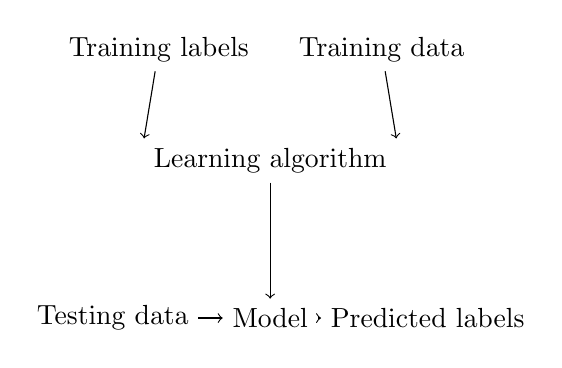
\begin{tikzpicture}[node distance=2cm, auto,]

    \node (model)  {Model};
    \node[right of=model] (predicted) {Predicted labels}
    	edge[<-] (model.east);
    \node[left of=model] (testing) {Testing data}
    	edge[->] (model.west);
    \node[above of=model] (learning_algo) {Learning algorithm}
    	edge[->] (model.north);
    \node[above right of=learning_algo] (t_data)   {Training data}
    	edge[->] (learning_algo.north east);
    \node[above left of=learning_algo]  (t_labels) {Training labels}
    	edge[->] (learning_algo.north west);

  \end{tikzpicture}
\end{document}